%==============================================================================
% Chapitre 61 - Les chevrotines
%==============================================================================

\section{Introduction}

Les chevrotines occupent une position intermédiaire entre les cartouches à
grenaille classique et les cartouches à balle unique.

Elles utilisent un nombre limité de projectiles de diamètre relativement
important.

\begin{aretenir}

Une cartouche à chevrotines contient plusieurs gros projectiles sphériques
propulsés simultanément.

\end{aretenir}

\section{Origine du terme}

Le terme « chevrotine » trouve son origine dans son utilisation historique pour
la chasse de certains animaux de taille moyenne.

Aujourd'hui, le terme désigne principalement des cartouches contenant plusieurs
projectiles sphériques de grand diamètre.

\section{Principe général}

Contrairement à la grenaille classique, composée d'un grand nombre de petits
projectiles, la chevrotine utilise généralement quelques projectiles seulement.

Leur diamètre est nettement supérieur à celui des plombs de chasse
traditionnels.

\section{Position entre grenaille et balle}

Les chevrotines peuvent être considérées comme une solution intermédiaire entre :

\begin{itemize}
    \item la grenaille ;
    \item la balle unique.
\end{itemize}

Elles combinent partiellement les caractéristiques de ces deux approches.

\begin{figure}[htbp]
\centering

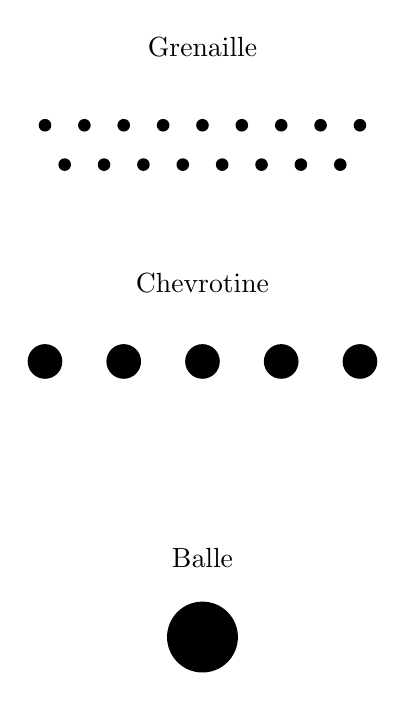
\begin{tikzpicture}

% Grenaille
\node at (0,3.5) {Grenaille};

\foreach \x in {-2,-1.5,-1,-0.5,0,0.5,1,1.5,2}
{
    \fill (\x,2.5) circle (0.08);
}

\foreach \x in {-1.75,-1.25,-0.75,-0.25,0.25,0.75,1.25,1.75}
{
    \fill (\x,2.0) circle (0.08);
}

% Chevrotine
\node at (0,0.5) {Chevrotine};

\foreach \x in {-2,-1,0,1,2}
{
    \fill (\x,-0.5) circle (0.22);
}

% Balle
\node at (0,-3.0) {Balle};

\fill (0,-4) circle (0.45);

\end{tikzpicture}

\caption{Comparaison simplifiée entre grenaille, chevrotine et balle unique.}
\label{fig:grenaille_chevrotine_balle}

\end{figure}

\section{Nombre de projectiles}

Selon le chargement, une cartouche à chevrotines peut contenir :

\begin{itemize}
    \item quelques projectiles ;
    \item plusieurs projectiles de grand diamètre ;
    \item des dispositions variables.
\end{itemize}

\section{Diamètre des projectiles}

Les projectiles utilisés sont généralement beaucoup plus gros que la grenaille
classique.

Cette augmentation du diamètre entraîne une augmentation importante de leur
masse.

\begin{figure}[htbp]
\centering

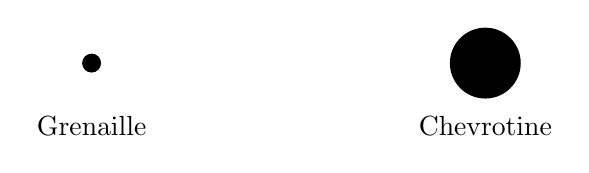
\begin{tikzpicture}

\fill (0,0) circle (0.12);

\node at (0,-0.8)
{Grenaille};

\fill (5,0) circle (0.45);

\node at (5,-0.8)
{Chevrotine};

\end{tikzpicture}

\caption{Comparaison qualitative entre un plomb de grenaille et une chevrotine.}
\label{fig:diametre_chevrotine}

\end{figure}

\section{Énergie individuelle}

Chaque projectile possède une énergie supérieure à celle d'un plomb de
grenaille classique.

Cette caractéristique influence fortement les effets obtenus.

\section{Dispersion}

Après la sortie du canon, les projectiles se dispersent progressivement.

La dispersion reste généralement plus faible que celle observée avec la petite
grenaille.

\section{Influence du choke}

Le comportement des chevrotines dépend également du choke utilisé.

Certaines combinaisons peuvent produire des résultats très différents selon les
armes.

\section{Essais pratiques}

Comme pour les autres cartouches de chasse, les essais sur cible restent
indispensables.

Ils permettent d'observer :

\begin{itemize}
    \item la dispersion ;
    \item la répartition ;
    \item la régularité.
\end{itemize}

\section{Applications historiques}

Les chevrotines ont été utilisées dans de nombreux contextes civils et
militaires au cours de l'histoire.

Leur emploi a varié selon les époques et les réglementations.

\section{Influence de la distance}

Lorsque la distance augmente :

\begin{itemize}
    \item la dispersion augmente ;
    \item la densité des impacts diminue ;
    \item la probabilité de toucher la cible évolue.
\end{itemize}

\begin{figure}[htbp]
\centering

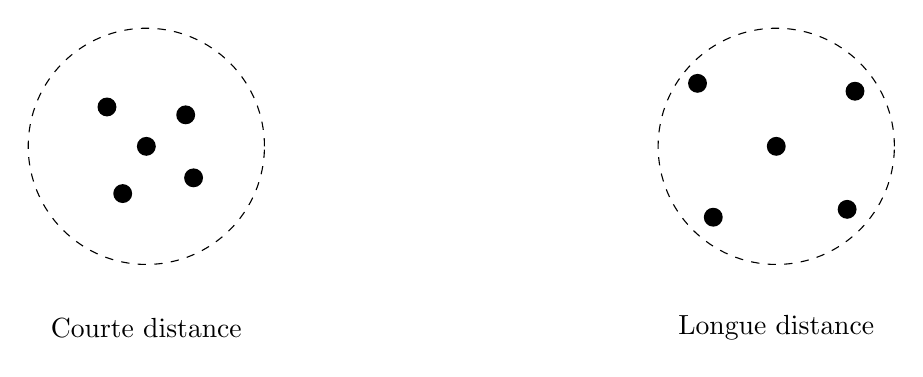
\begin{tikzpicture}

% Courte distance
\draw[dashed] (0,0) circle (1.5);

\foreach \x/\y in {
-0.5/0.5,
0.5/0.4,
0.0/0.0,
-0.3/-0.6,
0.6/-0.4
}
{
\fill (\x,\y) circle (0.12);
}

\node at (0,-2.3)
{Courte distance};

% Longue distance
\begin{scope}[xshift=8cm]

\draw[dashed] (0,0) circle (1.5);

\foreach \x/\y in {
-1.0/0.8,
1.0/0.7,
0.0/0.0,
-0.8/-0.9,
0.9/-0.8
}
{
\fill (\x,\y) circle (0.12);
}

\node at (0,-2.3)
{Longue distance};

\end{scope}

\end{tikzpicture}

\caption{La dispersion des chevrotines augmente progressivement avec la distance.}
\label{fig:dispersion_chevrotine}

\end{figure}

\section{Avantages}

Parmi les avantages souvent cités :

\begin{itemize}
    \item plusieurs projectiles ;
    \item énergie individuelle importante ;
    \item simplicité de mise en œuvre.
\end{itemize}

\section{Limites}

Les chevrotines présentent également certaines limites :

\begin{itemize}
    \item dispersion croissante avec la distance ;
    \item performances variables selon les armes ;
    \item dépendance aux réglementations locales.
\end{itemize}

\section{Comparaison avec la balle unique}

La balle unique concentre toute l'énergie dans un seul projectile.

La chevrotine répartit cette énergie entre plusieurs projectiles.

Ces deux approches répondent à des besoins différents.

\begin{figure}[htbp]
\centering

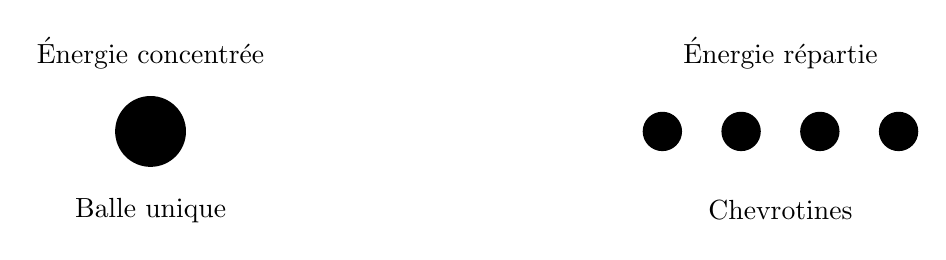
\begin{tikzpicture}

% Balle
\fill (0,0) circle (0.45);

\node at (0,-1)
{Balle unique};

\node at (0,1)
{Énergie concentrée};

% Chevrotines
\begin{scope}[xshift=8cm]

\foreach \x in {-1.5,-0.5,0.5,1.5}
{
    \fill (\x,0) circle (0.25);
}

\node at (0,-1)
{Chevrotines};

\node at (0,1)
{Énergie répartie};

\end{scope}

\end{tikzpicture}

\caption{La balle concentre l'énergie dans un seul projectile, la chevrotine la répartit entre plusieurs projectiles.}
\label{fig:energie_chevrotine}

\end{figure}


\section{Aspects réglementaires}

Les conditions d'utilisation des chevrotines varient selon les pays et les
contextes d'emploi.

Il convient toujours de se référer à la réglementation applicable.

\section{Vers les balles pour fusils lisses}

Les chevrotines représentent une étape intermédiaire entre la grenaille et les
projectiles uniques.

Le chapitre suivant examinera les principales balles utilisées dans les fusils
à canon lisse.

\begin{figure}[htbp]
\centering

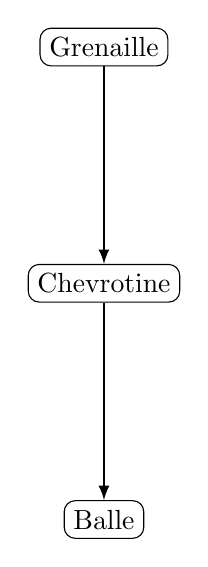
\begin{tikzpicture}

\node[draw,rounded corners]
(G)
at (0,0)
{Grenaille};

\node[draw,rounded corners]
(C)
at (0,-3)
{Chevrotine};

\node[draw,rounded corners]
(B)
at (0,-6)
{Balle};

\draw[-latex,thick]
(G)
--
(C);

\draw[-latex,thick]
(C)
--
(B);

\end{tikzpicture}

\caption{La chevrotine occupe une position intermédiaire entre la grenaille et la balle unique.}
\label{fig:position_chevrotine}

\end{figure}

\section{À retenir}

\begin{aretenir}

\begin{itemize}
    \item Les chevrotines utilisent plusieurs gros projectiles sphériques.
    \item Elles occupent une position intermédiaire entre grenaille et balle.
    \item Leur comportement dépend fortement de la distance et du choke.
    \item Les essais pratiques restent indispensables.
    \item Les réglementations peuvent varier selon les pays.
\end{itemize}

\end{aretenir}

\begin{figure}[htbp]
\centering

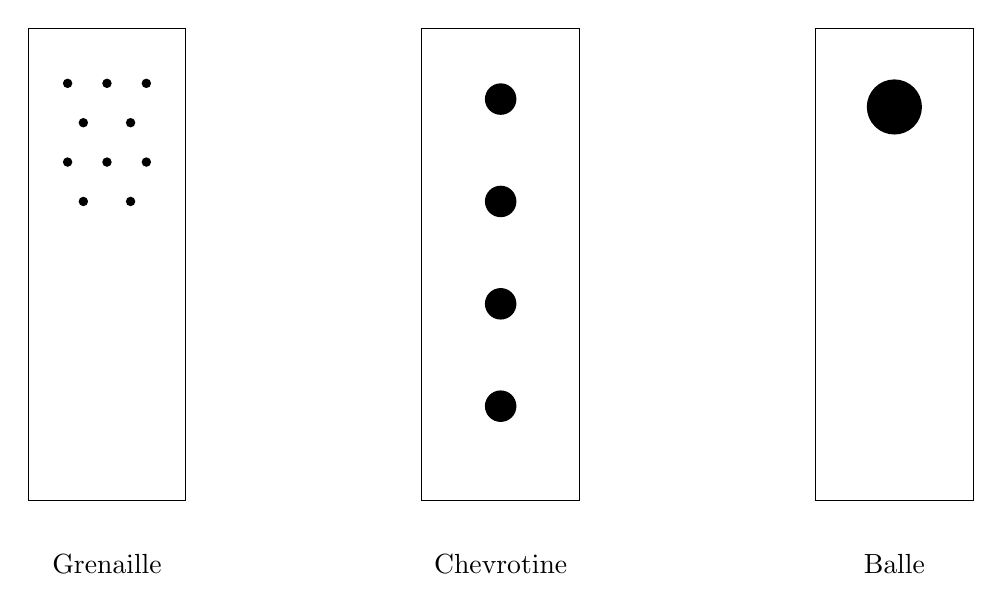
\begin{tikzpicture}

% Grenaille
\draw (0,0) rectangle (2,6);

\foreach \x/\y in {
0.5/5.3,1.0/5.3,1.5/5.3,
0.7/4.8,1.3/4.8,
0.5/4.3,1.0/4.3,1.5/4.3,
0.7/3.8,1.3/3.8
}
{
\fill (\x,\y) circle (0.06);
}

\node at (1,-0.8)
{Grenaille};

% Chevrotine
\begin{scope}[xshift=5cm]

\draw (0,0) rectangle (2,6);

\foreach \y in {1.2,2.5,3.8,5.1}
{
\fill (1,\y) circle (0.20);
}

\node at (1,-0.8)
{Chevrotine};

\end{scope}

% Balle
\begin{scope}[xshift=10cm]

\draw (0,0) rectangle (2,6);

\fill (1,5) circle (0.35);

\node at (1,-0.8)
{Balle};

\end{scope}

\end{tikzpicture}

\caption{Comparaison simplifiée du contenu de cartouches à grenaille, à chevrotines et à balle.}
\label{fig:contenu_cartouches}

\end{figure}
